\documentclass{standalone}
\usepackage{tikz}
\usetikzlibrary{angles, quotes}

\begin{document}
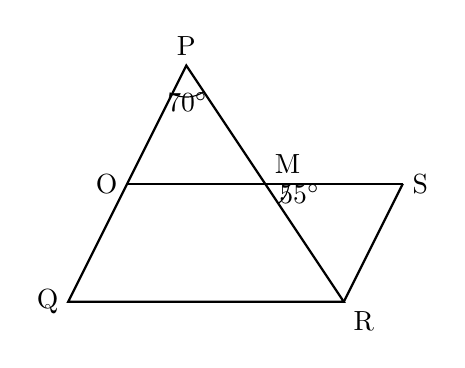
\begin{tikzpicture}[scale=1]
    % স্থানাঙ্ক নির্ধারণ (OQ || RS এবং OM || QR এর ভিত্তিতে)
    \coordinate (Q) at (0,0);
    \coordinate (R) at (3.5,0);
    \coordinate (O) at (0.75,1.5);
    \coordinate (S) at (4.25,1.5);
    
    % P বিন্দুটি QO এবং RM রেখা দুটির বর্ধিতাংশের ছেদবিন্দু
    \coordinate (P) at (1.5,3);
    
    % M বিন্দুটি PR এবং OS রেখার ছেদবিন্দু
    \coordinate (M) at (2.5,1.5);

    % মূল ত্রিভুজ PQR অঙ্কন
    \draw[thick] (P) -- (Q) -- (R) -- cycle;
    
    % OS এবং RS রেখা অঙ্কন
    \draw[thick] (O) -- (S);
    \draw[thick] (R) -- (S);

    % বিন্দুসমূহের লেবেল বা নাম প্রদান
    \node[above] at (P) {P};
    \node[left] at (O) {O};
    \node[left] at (Q) {Q};
    \node[above right] at (M) {M};
    \node[below right] at (R) {R};
    \node[right] at (S) {S};

    % কোণ ও মানসমূহ চিহ্নিত করা
    % P বিন্দুতে ৭০ ডিগ্রি কোণ
    \pic [draw, angle radius=0.4cm, "$70^\circ$" {shift={(0, -0.22)}}] {angle = Q--P--R};
    
    % M বিন্দুতে ৫৫ ডিগ্রি কোণ (RMS কোণ)
    \pic [draw, angle radius=0.3cm, "$55^\circ$" {shift={(0.28, -0.04)}}] {angle = R--M--S};

\end{tikzpicture}
\end{document}